%  Describe your problem and state your contributions.
\section{Introduction}
Road Segmentation is a category in semantic image segmentation tasks where the goal is to detect roads in aerial images. More specifically, given a set of labelled images, our task is to label each pixel as either road, or non-road, respectively. Challenges arise as parts of roads can be covered by trees or shadows of large buildings, resulting in fragmented predictions. Furthermore, roads can look considerably different in images taken at different locations or varying light conditions.

Since the success of \acrlong{cnn}s (\acrshort{cnn}s) in the 2012 ImageNet challenge \cite{imagenet}, \acrshort{cnn}s and its variants are widely applied. For such segmentation tasks, a particular encoder-decoder \acrshort{cnn} architecture, the U-Net \cite{unet}, has proven successful as it enables the precise localization of objects in an image. A remarkable research area focuses on extending the plain U-Net by proposing a slightly modified network structure or by adding new components. The Res-U-Net \cite{resunet}, for example, adapts the concept of residual learning \cite{residual} to introduce so-called residual blocks, and the \acrfull{gcdcnn} \cite{gcdcnn} in turn, makes use of dilated convolutions to further enlarge the receptive field.

However, not only are these variants increasingly complex to understand, they also require more sophisticated hyper parameter tuning and significantly longer training times. Therefore, we are posing the following research question: \emph{What is the contribution of these complicated network architectures in terms of prediction accuracy compared to alternative methods such as image augmentations, post-processing and using additional training data?}

%Original: What is the contribution of these complicated network architectures in terms of prediction accuracy compared to the contribution of pre- and  post-processing techniques and additional training data?

In our analysis, we show that by appropriate tuning, we can reach similar or even higher prediction accuracy, while requiring significantly less computing resources with the U-Net compared to the \acrshort{gcdcnn}. An example prediction can be seen in Figure \ref{fig:example}.

While fine tuning the baseline models, we extensively experimented with alterations to the model architecture itself especially for \acrshort{gcdcnn}. This lead us to a novel variant \acrshort{gcdcnn}-Plus which improved the baseline model. Additionally, we applied post-processing methods to remove recurring artefacts such as disjoint line segments, noisy images etc in the model predictions. Motivated by the idea that a human could heuristically connect line fragments just by looking at the predicted mask, we came up with two novel post-processing techniques.
%As an alternative to refining model architecture, we propose two novel post-processing techniques. 
One approach retrains the network on the binary predictions using partial convolution layers. Another approach makes use of Hough Transformations \cite{hough} to connect road fragments by completing lines and is motivated by the human behavior of annotating roads. Retraining on the binary predictions has improved prediction accuracy.

 \begin{figure}
 \centering
   \begin{subfigure}[b]{0.3\linewidth}
     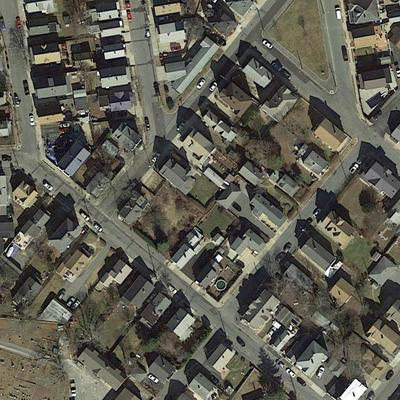
\includegraphics[width=\linewidth]{images/144_1_input_step_513.png}
     \caption{Input Image}
   \end{subfigure}
   %
   \begin{subfigure}[b]{0.3\linewidth}
     
\includegraphics[width=\linewidth]{images/144_2_true_step_513.png}
     \caption{True Label}
   \end{subfigure}
   %
   \begin{subfigure}[b]{0.3\linewidth}
     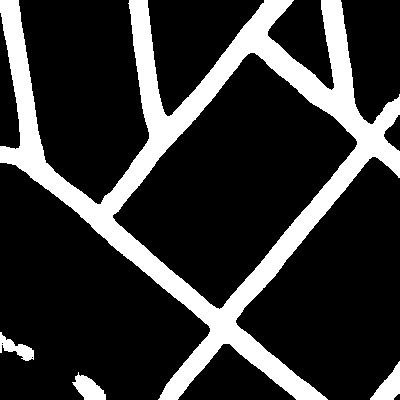
\includegraphics[width=\linewidth]{images/144_3_pred_epoch_073_step_38035.png}
     \caption{Prediction}
   \end{subfigure}
   \caption{Example image with prediction obtained from a U-Net trained on ETH-data, \textit{GMaps-public} and \textit{GMaps-custom}.} 
   \label{fig:example}
   \vspace{-6mm}
 \end{figure}

The remainder of this report is structured as follows: In Section \ref{section:data}, we describe the data we used and image augmentations we applied. Section \ref{section:models} presents our baseline models, describes the experiments we conducted to improve on these baselines and extensively elaborates on the contributions of model architecture. Our proposed post-processing techniques are explained and demonstrated in Section \ref{section:post}. Finally, results are compared in Section \ref{section:results} and discussed in Section \ref{section:discussion}.